\documentclass[a4paper, 11pt]{article}

\usepackage{caption}
\DeclareCaptionLabelFormat{adja-page}{\hrulefill\\#1 #2 {(see previous page)}}

\usepackage{graphicx}
\usepackage[export]{adjustbox}
\usepackage[left=1in,right=1in,top=1in,bottom=1in]{geometry}
\usepackage{xcolor}
\usepackage[bookmarksopen=true,pdfauthor=Lubos Polerecky,pdftitle=Look@NanoSIMS,pdfsubject=User manual]{hyperref}
\hypersetup{colorlinks=true,linkcolor=blue,urlcolor=blue}
\linespread{1.2}

\title{{\LARGE \bf Look@NanoSIMS}\footnote{\textbf{Citation}: L. Polerecky et al. (2012). Look@NanoSIMS --- a tool for the analysis of nanoSIMS data in environmental microbiology. \textit{Environmental Microbiology} 14 (4): 1009--1023. DOI: 10.1111/j.1462-2920.2011.02681.x}}
\author{\large\bf Lubos Polerecky\footnote{Feedback and questions can be sent to: l.polerecky@uu.nl}\\[3mm]
Max-Planck Institute for Marine Microbiology, Bremen, Germany (2002--2013)\\[2mm]
Department of Earth Sciences, Utrecht University, Utrecht, The Netherlands (2013--2025)}
\date{User's manual, version 28-06-2025\\[3mm]
\url{https://github.com/lpolerecky/LANS}}

\definecolor{darkgold}{RGB}{120,75,4}
\definecolor{darkgreen}{RGB}{4,120,4}
\definecolor{purple}{RGB}{128,0,128}
\newcommand{\ttt}[1]{\texttt{#1}}
\newcommand{\lans}[1]{{\color{magenta}#1}}
\newcommand{\lanscb}[1]{{\color{darkgreen}#1}}
\newcommand{\lanstf}[1]{{\color{cyan}#1}}
%\newcommand{<name>}[<args>]{ <code> }
\usepackage{marginnote}
\newcommand\mnote{\marginnote{\fbox{\textbf{\bf Note}}}}
\newcommand\ra{\rightarrow}
\newcommand\addon[1]{-- {\small #1}}

\begin{document}

\maketitle
\reversemarginpar 

%%

\section*{Summary}
\textbf{Look@NanoSIMS}, or shortly \textbf{LANS}, is a program for the analysis and processing of nanoSIMS data. Its primary aim is to be \emph{useful}.  The original development of the program started back in 2008, so in many aspects the program may be considered as an `old school'. However, based on input and requests from users, the program has been improved in many ways, and an active development continues until today. Over the years, the program has matured well and can now be used for many types of analysis of nanoSIMS data. This document describes how such analyses can be done at basic, intermediate and very advanced levels.

%%

\tableofcontents

\section{Installation instructions}

LANS is a Matlab-based program. Thus, a core \textbf{Matlab} installation, along with image processing and statistical toolboxes, is required to run LANS and perform basic functions. This makes it possible to run LANS on a variety of operating systems, including Linux, Microsoft Windows and MacOS. However, this also limits LANS to users with access to a Matlab license. Additionaly functionality of LANS is achieved by integrating the program with \textbf{\LaTeX} (for exporting results in a nicely formatted PDF output) and data compression programs such as \textbf{zip} (for decompressing input files and compressing output generated by LANS), both of which are available for free.

%%

\subsection{Install Matlab}

\begin{enumerate}

\item Matlab is available from \url{www.mathworks.com} and requires a license. It is useful to check whether your institution has a site-license (e.g., your university may have one for all students and academic staff). 

\item Version 2019b of Matlab is most recommended to ensure that all features of LANS work as designed. LANS works with newer Matlab versions as well, however, there is a risk that some functionality will issue errors due to less than perfect back-compatibility of Matlab.

\item When installing Matlab, you will need the \emph{core Matlab} and \emph{two toolboxes}: image processing and statistics and machine learning. 

\end{enumerate}

\mnote
Some output generated by LANS, e.g., information generated during the alignment of planes and stored in the file \ttt{xyalign.mat}, may not be read correctly by the Matlab version 2019b when it was generated by a newer Matlab version. Thus, if you plan to use LANS in collaboration with other people, e.g., by sharing the files generated by LANS among each other, it is recommended that everyone in the team uses the same Matlab version.

%%

\subsection{Install \LaTeX}

This software is required to enable export of graphical output as tagged PDF documents. 

\begin{enumerate}
 
\item To install \LaTeX, use one of the well-established \LaTeX\ distributions for your operating system, as described on the \href{https://www.latex-project.org/get/}{\LaTeX\ project} website (e.g., \ttt{texlive} for Linux, \ttt{MikTeX} for Windows, \ttt{MacTex} for MacOS). Note that the on-line LaTeX service, such as Overleaf, is insufficient; you really need a locally installed \LaTeX\ distribution.
 
\item To correctly integrate \LaTeX\ with LANS, you will need the following executables and packages installed and working:
 
\begin{itemize}
\item executables: \ttt{epstopdf}, \ttt{pdflatex}
\item packages: \ttt{graphicx}, \ttt{geometry}, \ttt{hyperref}
\end{itemize}
 
\end{enumerate}
 
\mnote
If you have never used \LaTeX\ on your computer, it may be that some \LaTeX\ packages, particularly \ttt{geometry} and \ttt{hyperref}, are not installed during the 'standard' installation procedure. As a result, the execution of the LANS functions \lans{Export LaTeX and PDF output} (main LANS) or \lans{Export images for each variable as PDF} (Process metafile) may get stuck if the packages are missing. If this happens, you can fix this problem by compiling the \ttt{tex} file using the native \LaTeX\ environment (e.g., open the \ttt{tex} file in the default editor of your \LaTeX\ distribution and then compile it into a \ttt{pdf} output from there). When doing so, the missing \LaTeX\ packages should automatically be installed and the \ttt{tex} file should compile into a correct \ttt{pdf} output. Once this is done, the automatic \LaTeX\ compilation from within Matlab will also work.

%%

\subsection{Install software for compressing/decompressing files}

This software is required for two reasons.

\begin{enumerate}
 
\item It enables you to load compressed nanoSIMS datasets (\ttt{im.zip} files) by LANS. This is a useful feature because \ttt{im.zip} files have roughly a 10-fold smaller size than the original \ttt{im} files generated by the Cameca's nanoSIMS measurement software. It is recommended to store and distribute the raw data files by first compressing them with the \ttt{zip} program (extension \ttt{im.zip}). 

\item It allows you to compress the processed data generated by LANS. This is convenient for making data backups, since it is much more efficient to upload and download few compressed folders than hundreds of smaller files present in those folders.

\item \ttt{7-Zip} (freeware) is recommended for Microsoft Windows. \ttt{zip} and \ttt{unzip} are available by default on Linux and MacOS systems.

\end{enumerate}

%%

\subsection{Install Look@NanoSIMS}

This is done by copying the source files to a folder on your computer.

\begin{enumerate}
 
\item For convenience, the compressed file containing the \emph{latest version of LANS} is stored in this \href{https://www.dropbox.com/sh/gyss2uvv5ggu2vl/AABViAmt9WHryEP_xZBrCG_La?dl=0}{Dropbox folder}. Click on the \ttt{program} folder and then download the file \ttt{LANS-latest-src.zip}.

\item Unzip \ttt{LANS-latest-src.zip} to a folder of your choice.

\item Rename the \ttt{src} folder using a more reasoname name (e.g., \ttt{LANS-2025-05-26}, where the data will refer to the LANS version).

\end{enumerate}

\mnote
In case the Dropbox link above does not work, because it became outdated or the official distribution location changed, visit the LANS' github repository or try to search the internet for more updated information. For users familiar with git and github, LANS can be downloaded by pulling the source code from the \ttt{src} folder in the LANS github repository: \url{https://github.com/lpolerecky/LANS}.

%%

\subsection{Starting Look@NanoSIMS for the first time}

Before you run LANS for the first time, revise the content of the files \ttt{lookatnanosims.m} and \ttt{lans\_paths.m}. These two files contain important settings you need to adjust to reflect your specific local installation of LANS. For example, you can specify there:

\begin{itemize}
\item locations of the compression/decompression software,
\item location of the PDF viewer,
\item default name of the file containing regions of interest (ROIs),
\item default extension of the raw data files.
\end{itemize}

\mnote
If you browse through the LANS installation files, you will notice that the \ttt{*.fig} files, which define the graphical user interface (GUI), appear in two sub-folders: \ttt{figs} and \ttt{figs\_win}. This is required because GUI defined on Unix-like and Windows platforms do not look the same. This is an issue due to --- apparently --- limited cross-platform compatibility of Matlab visual objects. It is not important for you as an end-user of LANS. You only need to be aware of it. Should you wish to modify any of the \ttt{*.fig} files, you will need to do it twice.

%%

\subsection{Starting Look@NanoSIMS on a regular basis}

\begin{enumerate}

\item Start Matlab.

\item Set the current folder to the folder where you installed LANS. You can do this through the menu or, more easily, entering one of the following commands in the Matlab console (the precise syntax depends on whether you use Windows, Linux or MacOS, and on the path where you installed LANS):

\ttt{>> cd c:/programs/LANS}

\ttt{>> cd /home/your\_username/programs/LANS}

\item Once you are in the correct folder, enter the following command in the Matlab console:

\ttt{>> lookatnanosims}

If everything is set up correctly, the main LANS graphical user interface (GUI) will open (Fig.~\ref{fig1:mainLANSgui}). You can start from there, as described in the following sections of this document. 

\end{enumerate}

\begin{figure}[!t]
\centering
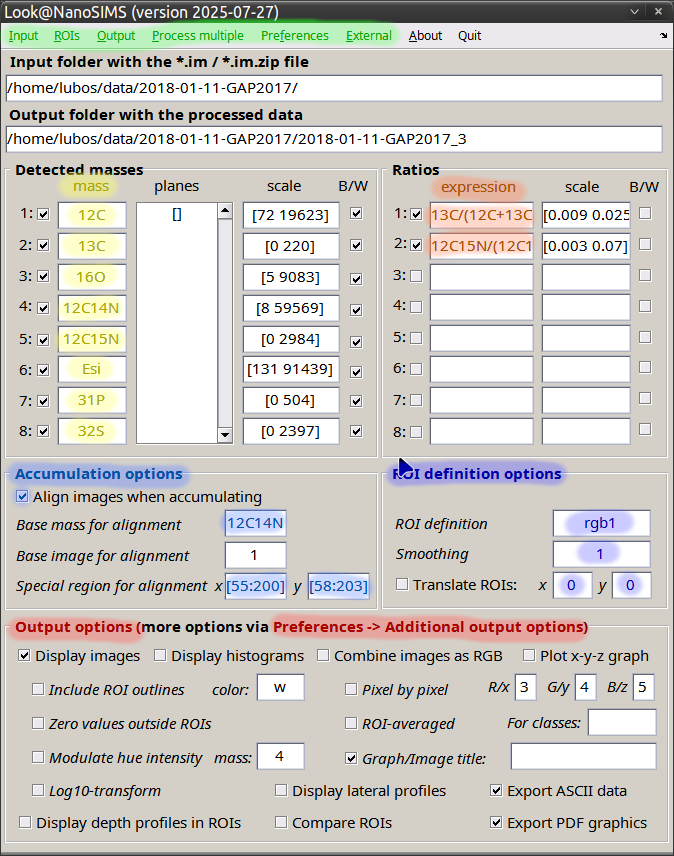
\includegraphics[width=0.9\textwidth]{figs1/LANS-maingui}
\caption{\label{fig1:mainLANSgui}%
Main graphical user interface (GUI) of Look@NanoSIMS.}
\end{figure}

\mnote
During the data processing session, LANS provides quite a lot of useful information in the Matlab console. Thus, it is a good idea to \emph{always} keep an eye on the output in the console. You can do this by arranging your desktop such that the LANS and Matlab console windows are \emph{both visible at the same time}. This is also useful in case you encounter an error while working in LANS. These errors will be shown in the console, too.


%%

\subsection{Updating Look@NanoSIMS}

\begin{enumerate}
 
\item LANS is updated quite regularly. You can update it easily by entering in the Matlab console:

\ttt{>> lans\_webupdate} 

You need to be in the folder where LANS is installed. You will be prompted to make a backup of your older LANS version, which is recommended to do, just in case.

\item If you are familiar with \ttt{git}, you can update LANS by pulling the latest sources from the LANS github repository \url{https://github.com/lpolerecky/LANS}.

\end{enumerate}

%%%%

\section{Organization of the input and output data}

Working with LANS, and with nanoSIMS data in general, can be a book-keeping challenge. To start with, you will have many raw data files (\ttt{im} or \ttt{im.zip} files) acquired at different dates and from different types of samples (e.g., different treatments). Additionally, processing of those raw data files with LANS will create many output files, including ASCII data, PDF images, matlab output, PDF output, and zipped backed-up folders. It is therefore a good idea to develop and maintain a certain structure of those folders and output files, to \emph{keep everything organized}. 

In this document, we assume that the raw and processed nanoSIMS data are organized hierarchically as shown in Table~\ref{tab1:file_structure}. We have used this data organization at Utrecht University for many years, and it works pretty well. We therefore highly encourage users to adopt it as well. Its benefits will become more apparent later on, when we get to the point of explaining how to efficiently process and analyze \emph{multiple} nanoSIMS datasets from a particular project.

\begin{table}[ht]
\centering
\caption{\label{tab1:file_structure} Hierarchical organization of the raw and processed nanoSIMS data implemented in Look@NanoSIMS. An example of such data organization along with a more detailed explanation is shown in Fig.~\ref{fig2:data_organization}.}
\begin{tabular}{l@{ $\rightarrow$ }c@{ $\rightarrow$ }l@{ $\rightarrow$ }l@{ $\rightarrow$ }l}
\hline
root & project & measurment day 1 & raw dataset 1.1 & \color{red}{dataset folder} 1.1\\
\multicolumn{2}{c}{} & & raw dataset 1.2  & dataset folder 1.2\\
\multicolumn{2}{c}{} & & $\cdots$ & $\cdots$ \\
\multicolumn{1}{c}{} & & measurement day 2 & raw dataset 2.1  & dataset folder 2.1\\
\multicolumn{2}{c}{} & & raw dataset 2.2  & dataset folder 2.2\\
\multicolumn{2}{c}{} & & $\cdots$ & $\cdots$\\
\multicolumn{1}{c}{} & & $\cdots$ & $\cdots$ & $\cdots$\\
\hline
\multicolumn{2}{r}{\color{red}{dataset folder} $i$ $\rightarrow$} & \color{orange}{dat} & \multicolumn{2}{l}{\color{orange}{numbers}} \\
\multicolumn{2}{r}{$\rightarrow$} & \textcolor{darkgold}{pdf} & \multicolumn{2}{l}{\textcolor{darkgold}{images \&\ graphs}} \\
\multicolumn{2}{r}{$\rightarrow$} & \multicolumn{3}{l}{\hspace{-2mm}processing definition files (\textcolor{purple}{alignment, ROIs, preferences})} \\
\multicolumn{2}{r}{$\rightarrow$} & \multicolumn{3}{l}{\hspace{-2mm}\textcolor{purple}{OutputG.pdf (output summary)}}\\
\hline
\end{tabular}
\end{table}

At the highest level of the data organization is a root folder that contains \emph{all} nanoSIMS data. This folder contains `project folders' with nanoSIMS data belonging to \emph{specific projects}. Each `project folder' contains `day folders' with data acquired on \emph{different measurement days}. Each `day folder' contains the actual \emph{raw datasets} (\ttt{im} or \ttt{im.zip} files). When a particular raw dataset is processed and analyzed, the corresponding data is stored in a `dataset folder' with the \emph{same name} as the dataset. Each `dataset folder' contains sub-folders with the \emph{results} of the analysis, including numerical values such as ROI-specific ion counts or ion count ratios (folder \ttt{dat}), and graphical output such as images or scatter plots (folder \ttt{pdf}). The `dataset folder' also contains information defining the processing steps, such as alignment of frames, definition and classification of regions of interest (ROIs), and preferences. This information is useful if you want to go back to the analysis of the same dataset after you have analyzed a different one, e.g., to perform quality checks or more in-depth analyses. Finally, the `dataset folder' also contains a PDF file with a comprehensive graphical summary of the analysis. This file is useful if you wish to share the results for a specific dataset with project collaborators.


\begin{figure}[b!]
\centering
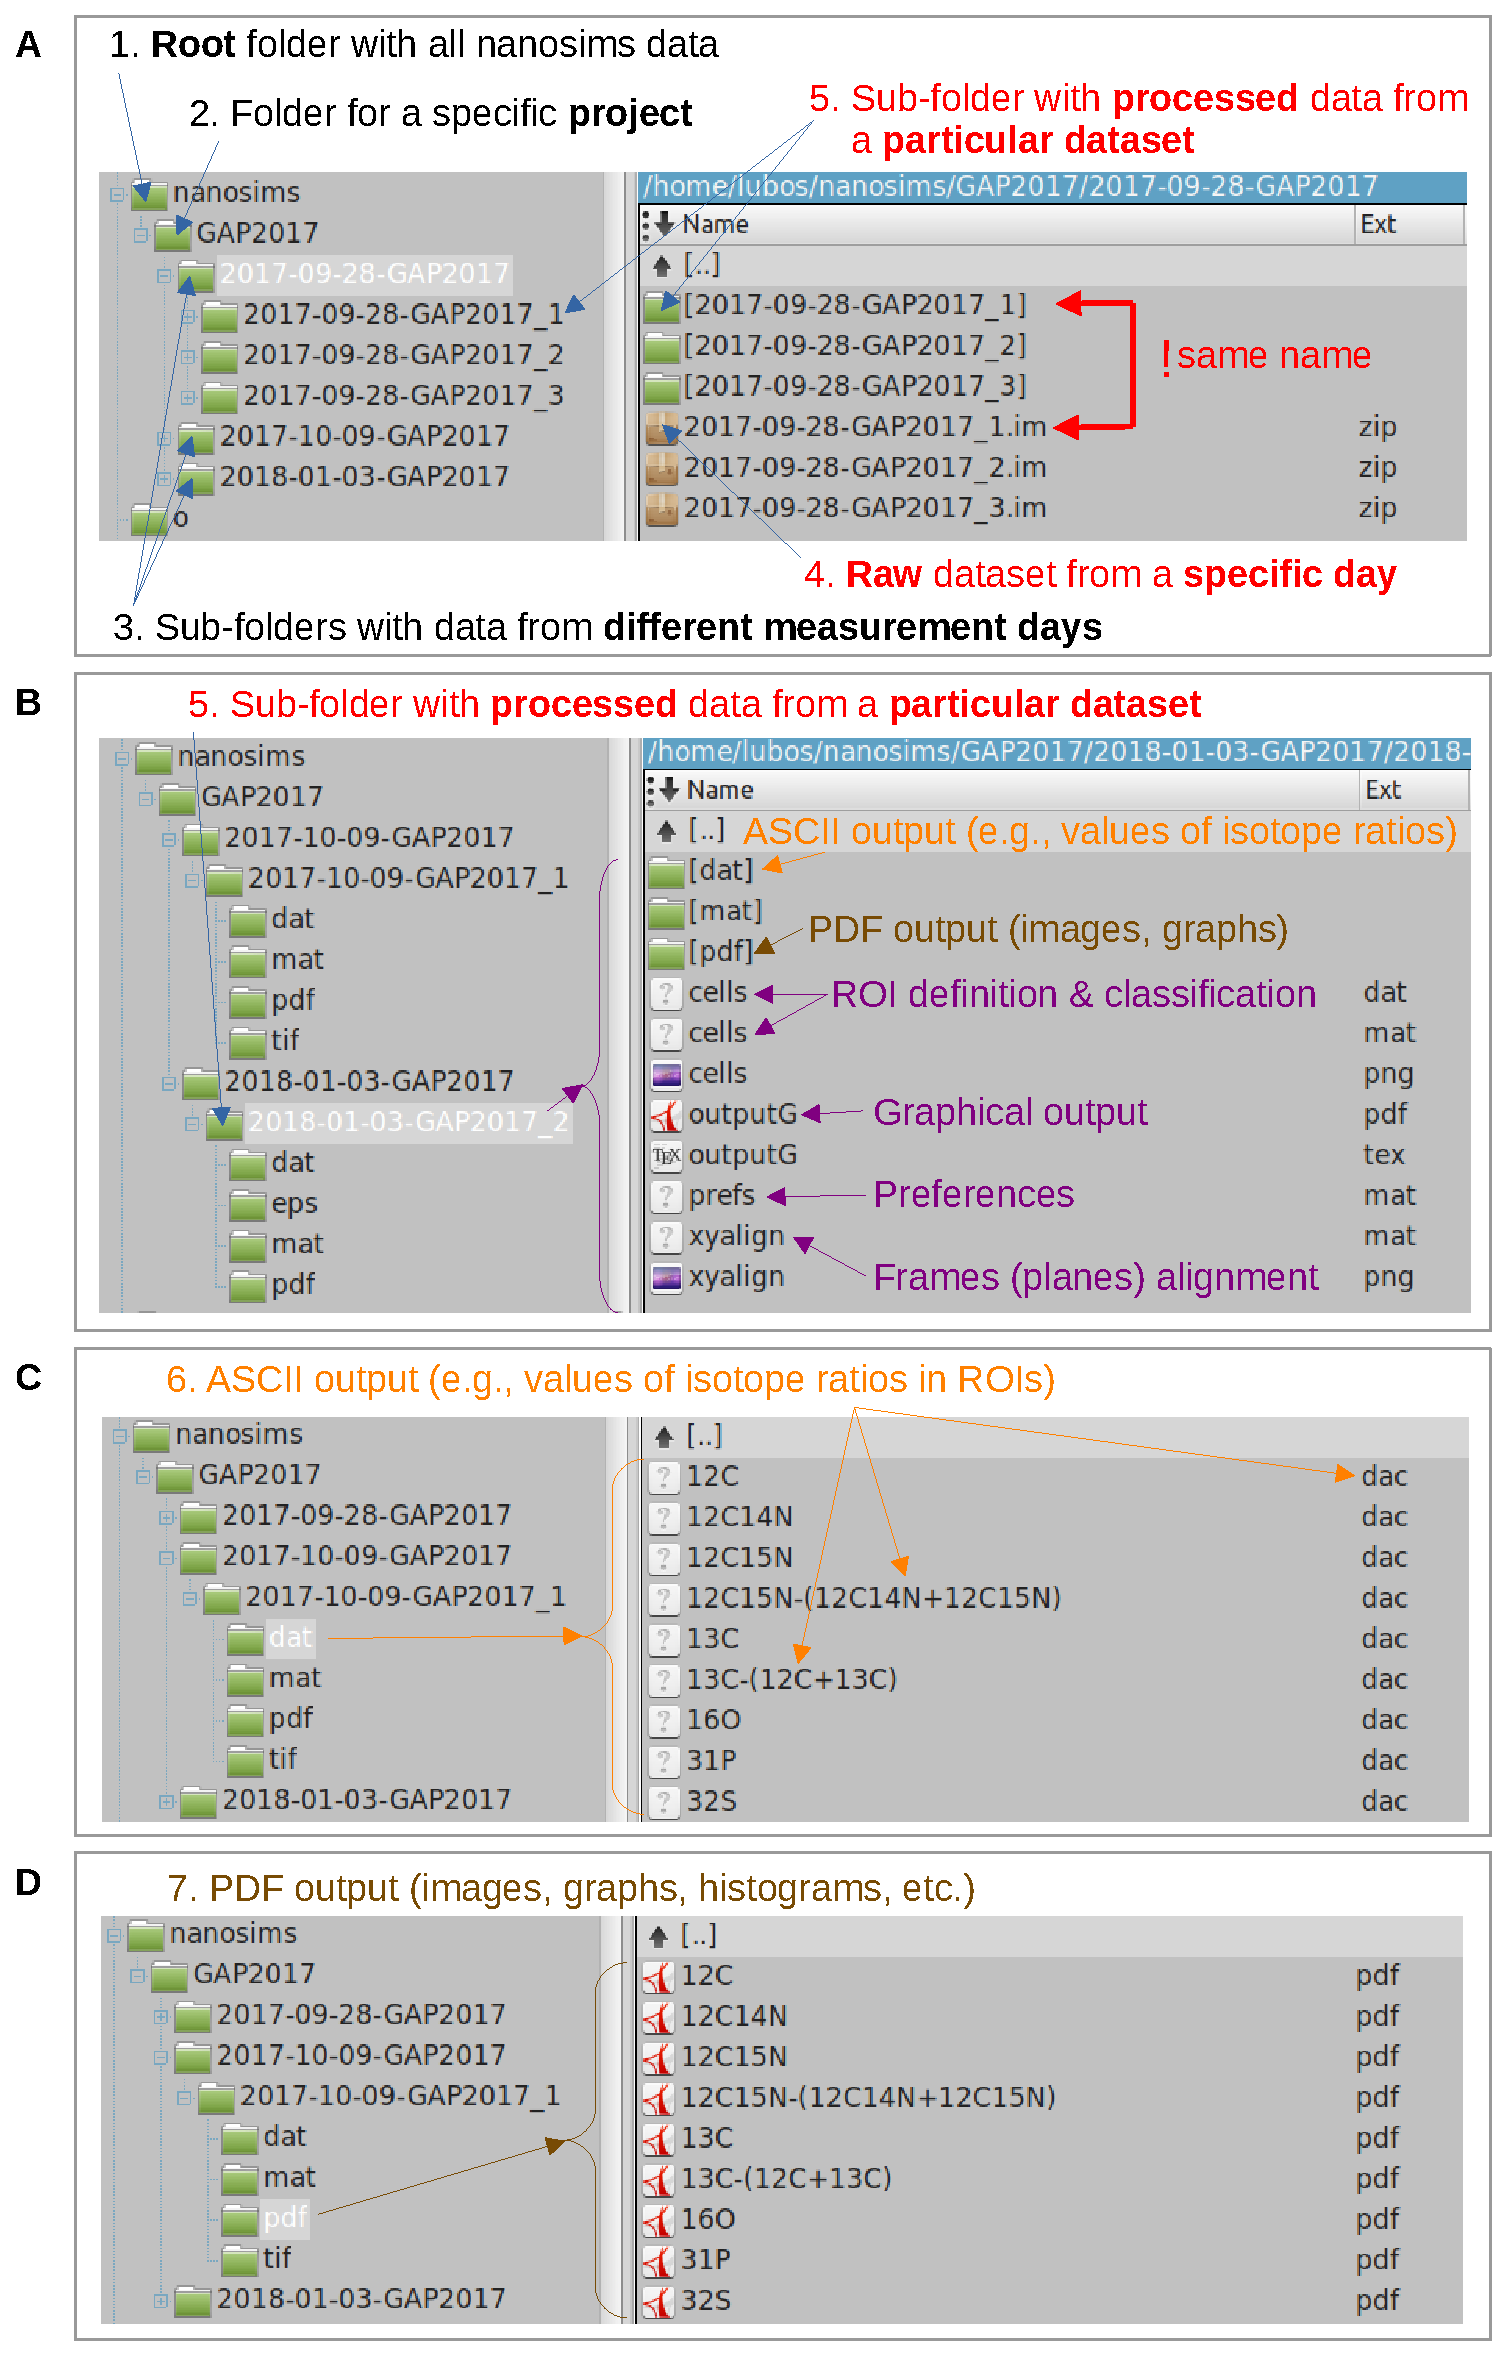
\includegraphics[height=0.97\textheight]{figs2/folders_organization}
\caption[]{(see next page)}
\end{figure}
\begin{figure} [t!]
    \captionsetup{labelformat=adja-page}
    \ContinuedFloat
    \caption[Figure]{%
    Example of a hierarchical organization of the raw and processed nanoSIMS data implemented in Look@NanoSIMS. %
    \textbf{(A)} The root folder (\ttt{nanosims}) contains a~project-specific sub-folder (\ttt{GAP2017}), which contains sub-folders with data measured on different days (e.g., \ttt{2017-09-28-GAP2017}, \ttt{2017-10-09-GAP2017}). %
    The `day folder' contains \emph{multiple raw datasets} measured on that particular day (\ttt{im} or \ttt{im.zip} files). %
    When a particular raw dataset is processed and analyzed, the data is stored in a `dataset folder' with the \emph{same name} as the dataset (see red `!'). %
    \textbf{(B)} The `dataset folder' contains files defining the processing steps, including alignment information (\ttt{xyalign}), definition and classification of regions of interest (\ttt{cells.mat} and \ttt{cells.dat}, respectively), preferences (\ttt{prefs.mat}), and a comprehensive summary of results exported in a PDF file (\ttt{OutputG.pdf}). %
    The `dataset folder' also contains sub-folders with ASCII (\ttt{dat}), PDF (\ttt{pdf}) and Matlab (\ttt{mat}) output. %
    \textbf{(C)} The \ttt{dat} folder contains the ROI-specific ion counts and ion count ratios (\ttt{dac} files). %
    \textbf{(D)} The \ttt{pdf} folder contains the exported images, graphs, histograms, etc. }
    \label{fig2:data_organization}
\end{figure}

%%

\section{Data processing with Look@NanoSIMS --- quick summary}

This section provides a quick summary of steps taken during a typical data processing session. Refer to Sections~\ref{sec:level1}, \ref{sec:level2} and \ref{sec:level3} for more details, depending on the level of analysis. Throughout this document, we will use colored text when refering to a specific \lans{menu item or action button}, \lanscb{checkbox} or \lanstf{text field} in the program's GUI.


\subsection{Analysis of a single dataset --- ``from scratch''}

\begin{enumerate}

\item We start from the \lans{Input} menu. Define \lans{dead-time and QSA correction settings}.

\addon{Usually, these corrections are not necessary and this step can be skipped.}

\item \lans{Load RAW dataset} from disk. 

\addon{Before you do this, click on \lans{Ask for range of planes and mases before loading} if you want to select specific planes and masses when loading the raw data from disk. This may be useful if your dataset is huge (e.g., more than 1~GB of data) and the memory (RAM) on your computer is insufficient.}

\item \lans{Autoscale plane images} to set the scale for all masses automatically. 

\item \lans{Display plane images for all masses} to view the raw data as scaled images, plane by plane and in linear or log scale. 

\addon{In this step, you will be able to decide which mass will be used as a \lanstf{base mass for alignment} of planes during accumulation.}

\item Define \lanstf{base mass for alignment} and then select \lans{display alignment mass} to check the data plane by plane. 

\addon{While viewing the data, \lanscb{deselect planes} that should be excluded from accumulation (e.g., if the data in that plane is corrupt).}

\addon{At the end of this checking, \lans{define alignment region} within the image. This region will be used when calculating misalignment between subsequent planes. }

\item \lans{Accumulate plane images} to accumulate ion counts over all selected planes.  

\addon{Before you do that, check \lanscb{align images when accumulating} if you do want to perform drift-correction of planes during accumulation.}

\mnote
\addon{At the end of automatic drift-correction, you will be prompted to accept or reject the drift-correction information. If you \lans{accept}, the information will be stored in the file \ttt{xyalign.mat} and all planes for all masses will be accumulated based on this information. If you \lans{reject}, you can reiterate steps 4--6 until you arrive at a dataset with accumulated planes. If, anytime at a later point during your data analysis, you realize that you are not satisfied with the drift-correction, you need to first delete the \ttt{xyalign.mat} file (\lans{Preferences} $\ra$ \lans{Remove xyalign.mat from disk}) and then repeat steps 2--6.}

\item \lans{Autoscale accumulated images} and then \lans{display accumulated images for all masses} to view the accumulated ion count images for all masses. 

\addon{This will export the results in a PNG file. You can choose whether you want to display the ion counts in a linear or log scale by checking \lanscb{Log10-transform}.}

\item \lans{Output} $\ra$ \lans{Display masses} to display the accumulated images for all masses.

\addon{Before you do that, check \lanscb{Display images} and \lanscb{Export PDF graphics} checkboxes in the \ttt{Output options} area of LANS (at the bottom of the main GUI). The latter option is needed if you want to export the results as PDF.}

\mnote
\addon{You can tweak the appearance of the images, and many more output options, via \lans{Preferences} $\ra$ \lans{Additional output options}.}

\item \lans{Output} $\ra$ \lans{Display ratios} to display ratio images derived from the accumulated ion count images.

\addon{Before you do that, type \lanstf{expressions} and \lanstf{scales} for ratio images in the corresponding text fields. Also, do not forget to check \lanscb{Export PDF graphics}.}

\item Define regions of interest (ROIs) using \lans{ROIs} $\ra$ \lans{INTERACTIVE ROIs definition tool}.

\addon{Typically, much of nanoSIMS data analysis revolves around ROIs.}

\addon{Before you open the ROIs definition tool, specify the \lanstf{ROI definition template}.  This can be an individual mass, ratio, an RGB overlay of masses or ratios, or an external image.}

\addon{If an external image is chosen as a ROI definition template, it needs to be first aligned with the nanoSIMS image, which can be done via the \lans{External} menu (part of advanced analysis).}

\item \lans{Export ROIs image as graphics} to export the ROI outlines as PDF. 

\addon{This will also include a~unique identification numbers for each ROI.}

\item Select \lans{ROIs} $\ra$ \lans{Classify} to classify the defined ROIs. 

\addon{It is often useful to classify the ROIs. This can be done \lans{manually} or \lans{automatically} based on ROI-specific information.}

\item The type of subsequent analysis and result visualization depends on the options selected in the \ttt{Output options} area of LANS. For example, you can display \lanscb{images}, \lanscb{depth profiles in ROIs}, \lanscb{lateral profiles}, or \lanscb{histograms}. You can also \lanscb{combine images as RGB} overlays, \lanscb{plot x-y-z graphs} (scatter plots), or \lanscb{compare ROIs} using simple statistical methods. 

After you define your choices, the analysis is done by selecting \lans{Output} $\ra$ \lans{Display masses} or \lans{Display ratios}. 

\addon{Ensure that the checkboxes \lanscb{Export ASCII data} and \lanscb{Export PDF graphics} are checked if you want the results to be exported as numbers and images.}

\mnote
\addon{Displaying depth profiles of ion counts and ion count ratios in ROIs can be useful as a quality check of the data.}

\addon{When displaying images, you can \lanscb{log-transform} the values, \lanscb{include ROI outlines}, or \lanscb{modulate the hue} based on a specific combination of masses (part of advanced analysis).}

\addon{When exploring RGB overlays, including images and scatter plots, you can do so on a \lanscb{pixel-by-pixel} level or as \lanscb{ROI-averaged}.}

\item Select \lans{Output} $\ra$ \lans{Generate LaTeX + PDF output} to export results of your analysis in a comprehensive PDF file. 

\mnote
\addon{If you check \lanscb{View PDF after export} (available via \lans{Preferences} $\ra$ \lans{Additional output options}) and correctly set the \ttt{PDF\_VIEWER} variable (in the \ttt{lans\_paths.m} file), the PDF output will automatically be displayed after it has been generated. This can be convenient if you want to quickly see the results summary in a nicely organized way.}

\item Select \lans{Preferences} $\ra$ \lans{Store preferences} to save the settings of the current data processing session (we recommend to use the file name \ttt{prefs.mat}).

\mnote
\addon{This should be the last step of processing of an individual dataset. We emphasize that you do this, because this file will be \emph{very useful} if you want to re-process the current dataset in the future.}

\addon{Specifically, the file contains all information for the currently processed dataset that you see in the GUI, including the detected masses, planes selected for alignment, formulas for ion count ratios, scales, all output options, etc.}

\end{enumerate}

%%

\section{Data processing with Look@NanoSIMS --- basic level}
\label{sec:level1}

%%

\section{Data processing with Look@NanoSIMS --- intermediate level}
\label{sec:level2}

%%

\section{Data processing with Look@NanoSIMS --- advanced level}
\label{sec:level3}

\end{document}
